\section{Pseudo-data generation}
\label{section:pseudo-data}

The analysis strategy is shown in the flowchart in Figure~\ref{eflow}. This appendix shows the multiple possible options for 
creating background only pseudo-data mentioned in the flowchart. 4 options have been discussed here, two of them are
based on the untagged dijet data used in the already published inclusive dijet Run-2 search~\cite{Nishu:2646455} and the other two are entirely based on Monte Carlo.
For the ones based on the untagged dijet data, the analysis selection for the current iteration of the analysis 
was compared to the previous one and it was confirmed that we are using a subset of the standard inclusive dijet selection from 
previous iteration with an additional cut on $\eta$ and qg tagging specific cuts.

\subsection{Possible Options for Creating Pseudo-data}
\subsubsection{Option 1}
The first option here starts with using untagged dijet data using the selection for the current round of analysis. 
This untagged dijet data is to be fitted with 5 (or 6) parameter global fit
function. Then the fraction of events passing 1 or 2 gluon tag selection are then computed from MC. These fractions are then smoothed to 
get rid of any statistical fluctuations. These smoothed tagging effciencies are then to be applied to the fitted untagged data to obtain the pseudo-data. 
%A pictorial representation of this can be seen in Figure~\ref{}.

\subsubsection{Option 2}
This also starts with using untagged dijet data using the selection for the current round of analysis. 
This untagged dijet data is to be fitted with 5 (or 6) parameter global fit. To obtain the fraction of events
passing 1 or 2 gluon selection, an ABCD method is to be used. Here the per event tagging efficiencies
are obtained from a \ystar\ inverted region (using \ystar\ < 0.8). These are then smoothed to get rid of the 
statistical fluctuations, and applied to the fitted untagged data to obtain the pseudo-data.  
%A pictorial representation of this can be seen in Figure~\ref{}.

\subsubsection{Option 3}
This option relies entirely on Monte Carlo sample. First the inclusive selection (without q/g tagging specific cuts)
is applied to the MC. The fraction of events passing 1 and 2 gluon selection are obtained from the MC sample as well. These
fractions are then smoothed as in the previous two options, and then applied to the untagged dijet MC to obtain the pseudo-data.
%A pictorial representation of this can be seen in Figure~\ref{}.

\subsubsection{Option 4}
This option uses the MC with all selection cuts applied including the q/g tagging selection. 
A smoothing is to be applied to this spectrum in this case and this would need to be revisited 
in case the fitting fails to make sure our pseudo-data is always $N_{param+1}$.
%A pictorial representation of this can be seen in Figure~\ref{}.
This option suffers from lack of statistics, along with being entirely based on MC and is thus of least preference. 

\subsection{Pseudo-data for 1 gluon and 2 gluon tag categories}
This section give details about the pseudo-data used for the fit validation studies.
We have used Option 1 to create this pseudo-data as discussed in previous section. The $m_{jj}$ spectrum was
obtained using full Run-2 data with the following selection cuts:

\begin{itemize}
\item Trigger: Passes the lowest unprescaled single-jet trigger, HLT\_j420
\item Jet preselecton: Leading jet $\pt\ge 380\,\GeV$ and Jet multiplicity $\ge 2$
\item $|\Delta\phi|$ between 2 jets: $|\Delta\phi| > 1.0$
\item $|\ystar|$ between 2 jets: $|\ystar|<0.8$
\item \mjj\: \mjj\ > 1200\,\GeV 
\item $|\eta|$ for both jets: Jets must be fully within the tracking acceptance ($|\eta|<2.1$)
\end{itemize}

This spectrum is then fitted with 5 parameter global fit using Minuit2. Figure~\ref{fig:mjjFit_ystar0p8} shows the fitted spectrum.
To obtain the fraction of events passing one gluon tag selection from the inclusive
spectrum, same selection as mentioned above has been applied to the Pythia dijet MC samples.
Figure~\ref{fig:fraction_1gtag_unsmooth} shows these fractions for one gluon tag category.

 \begin{figure}[!htb]
   \centering
   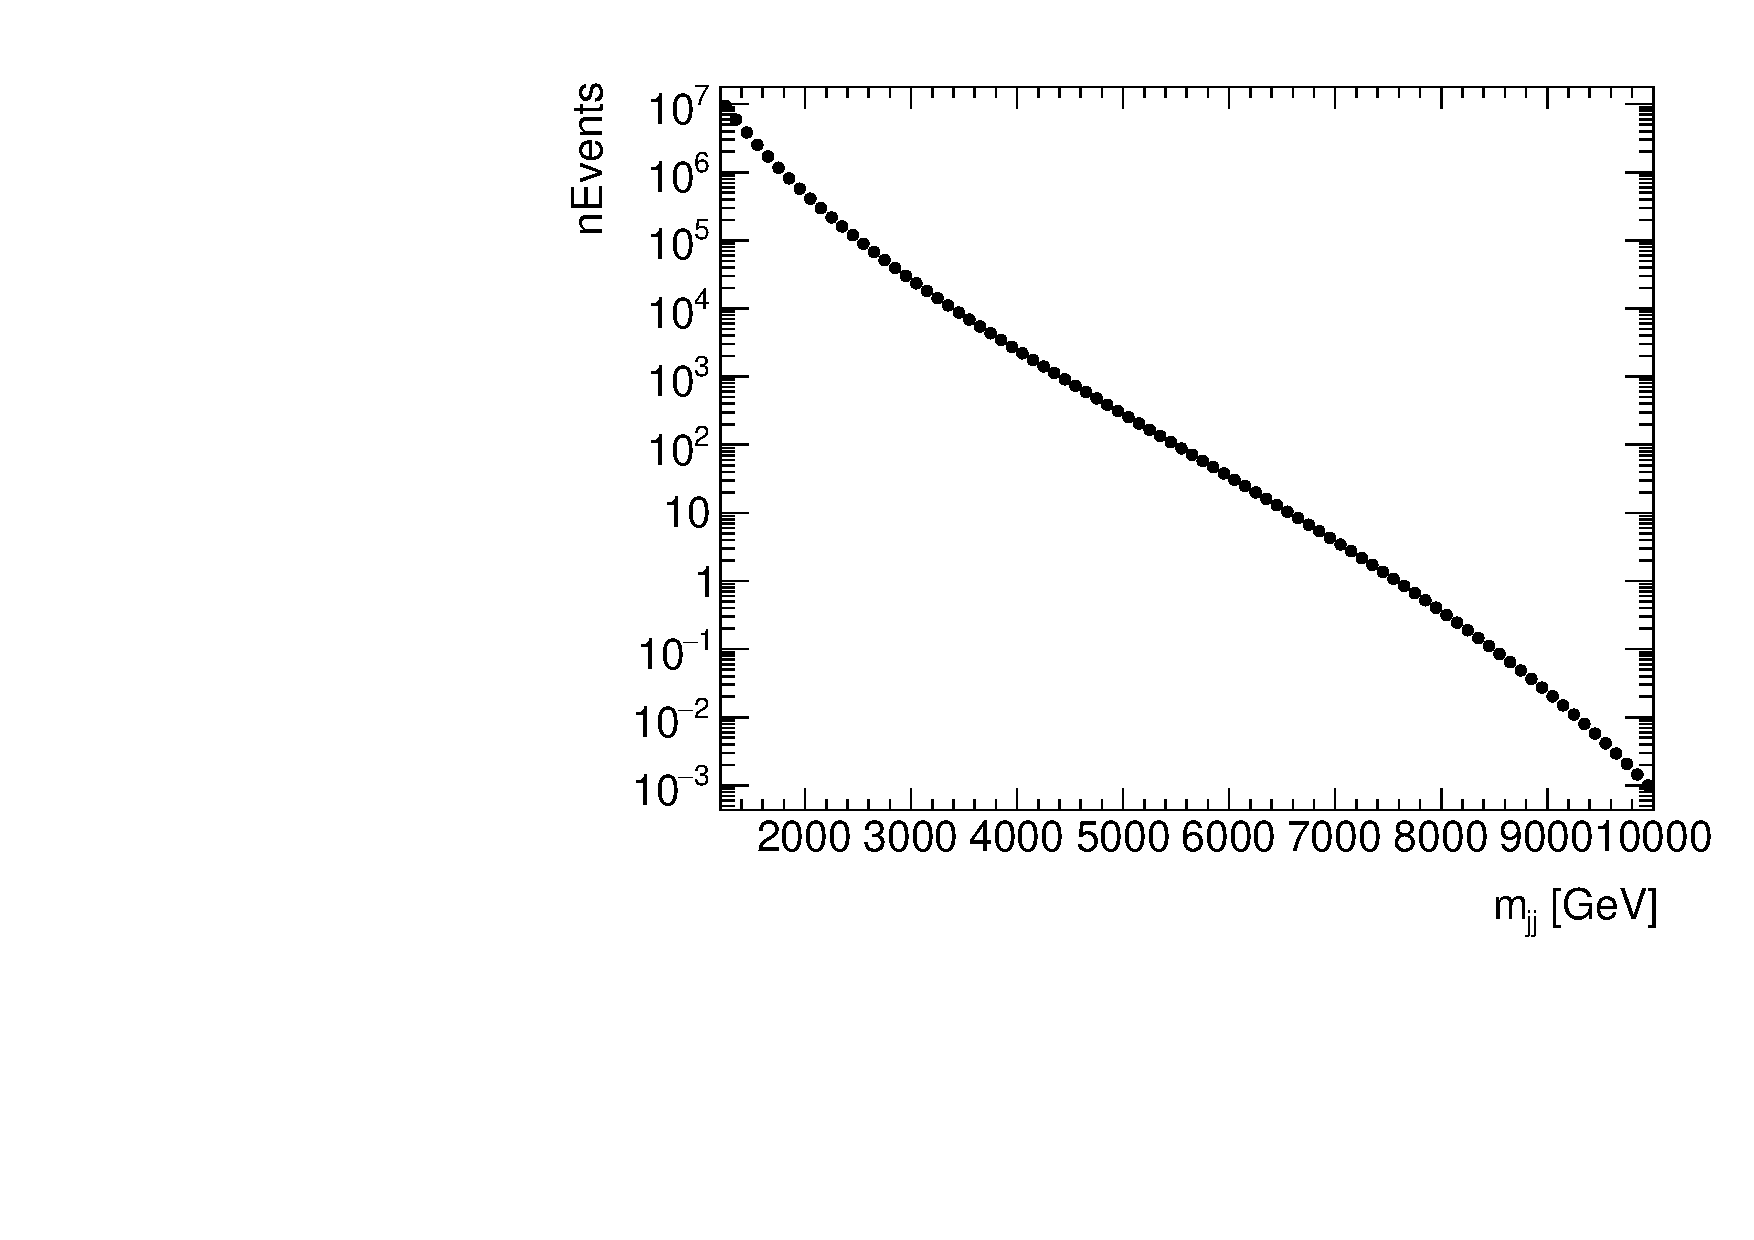
\includegraphics[width=0.45\textwidth]{figures/pseudodata/FittedMjj_UntaggedData_yStar0p8}
   \caption{Untagged dijet spectrum with $|\ystar|<0.8$ using Full Run-2 data fitted with 5 parameter global fit.
   \label{fig:mjjFit_ystar0p8}}
 \end{figure}

 \begin{figure}[!htb]
   \centering
   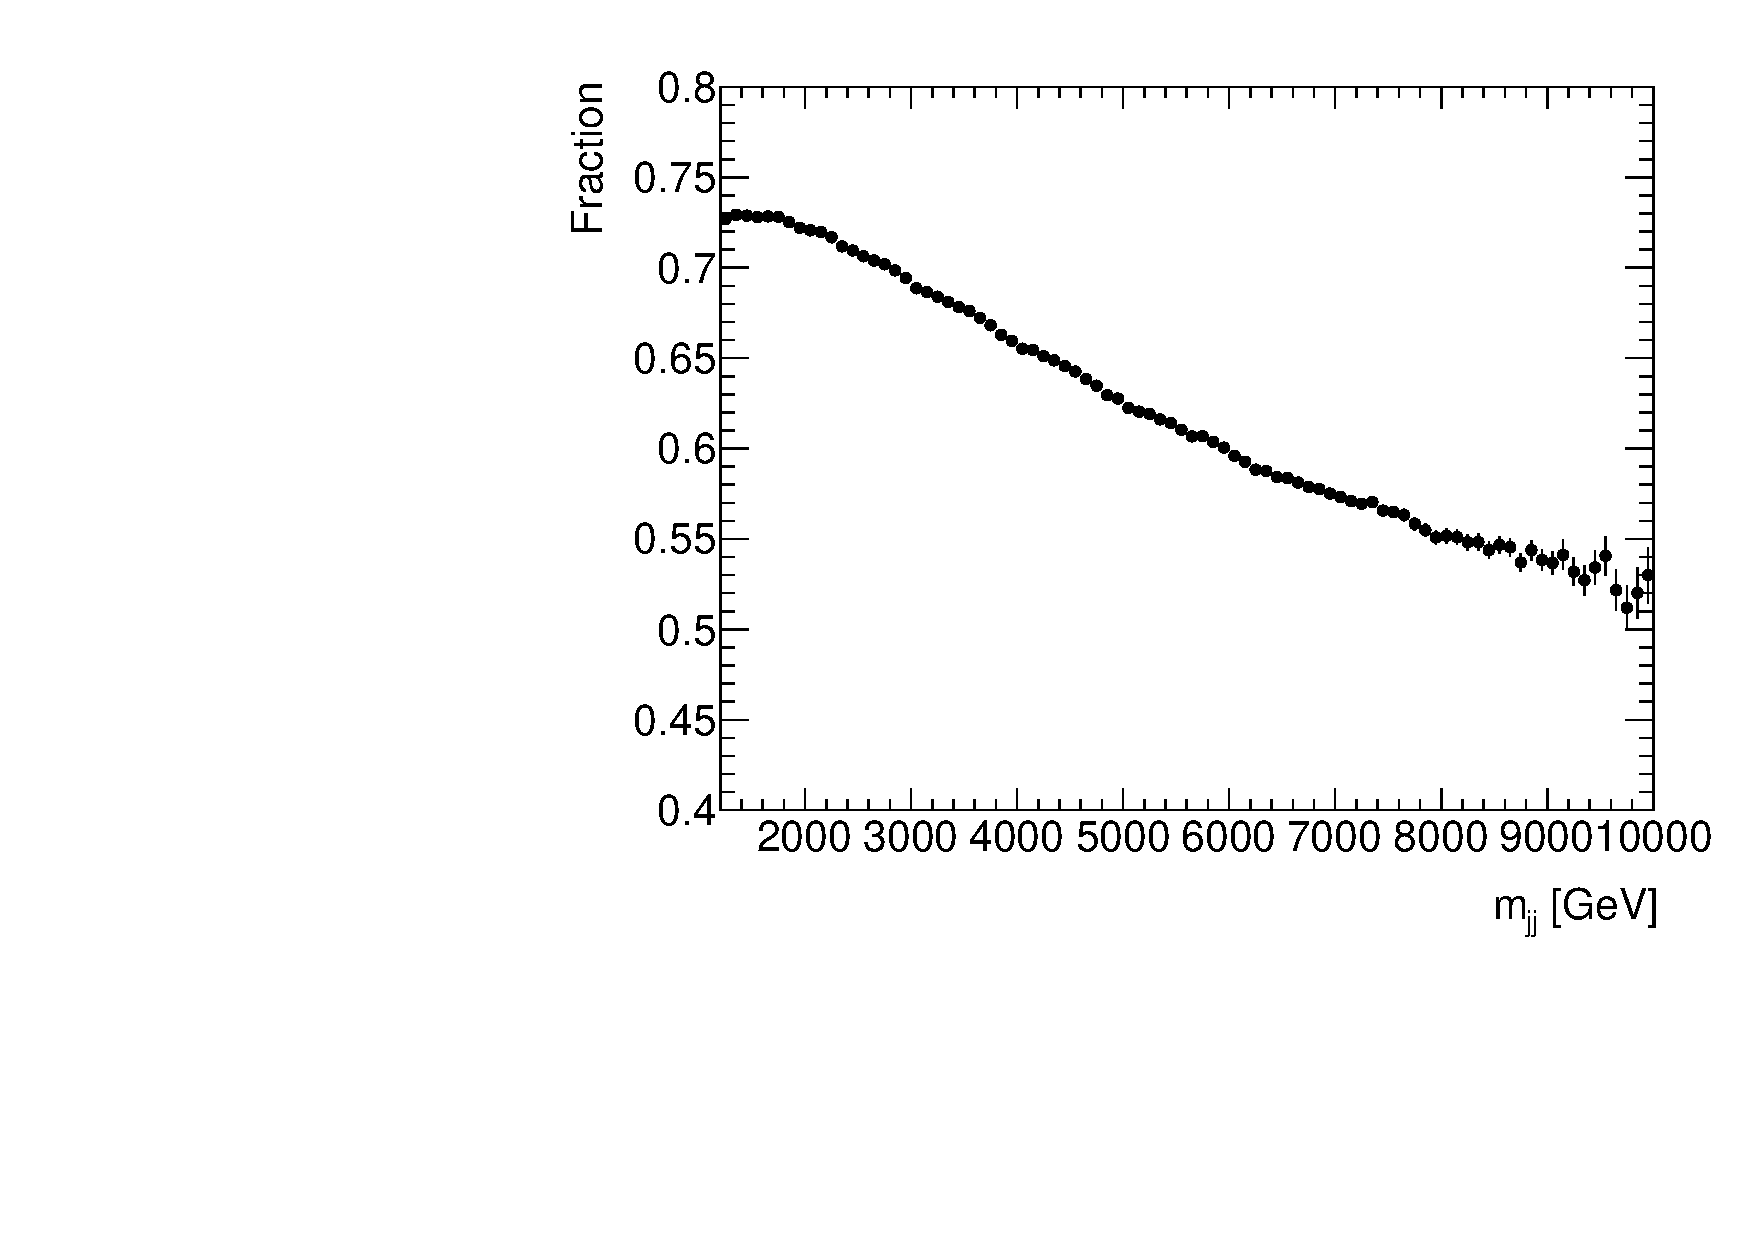
\includegraphics[width=0.45\textwidth]{figures/pseudodata/FractionUnsmooth_1gtag_yStar0p8}
   \caption{Fraction of events passing 1 gluon tag selection.
   \label{fig:fraction_1gtag_unsmooth}}
 \end{figure}


To smooth these fractions, a smoothing based on Friedman's SuperSmoother: https://github.com/
jakevdp/supersmoother has been used. Supersmoother is a non-parametric locally-linear smooth in which the size of the local neighborhood is tuned 
to the characteristics of the data. The degree of smoothing can be tuned with the bass enhancement feature.
This is a number (alpha) which lies between 0 and 10, with 10 being a much smoother curve. Different options were tried
for this smoothing parameter, with the ratios to the unsmoothened fractions obtained. Figure~\ref{fig:smoothFractions_1gtag} shows 
the smoothed fractions along with the comparisons to the unsmoothed fractions. It was seen that larger smoothing 
parameter gives much smoother curve but leads to some shape differences in the ratio plots, so a compromise between the two 
has been used. Some tests with BumpHunter were also performed to evaluate the differences between these different 
smoothing parameters. The very high vales of smoothing parameter (9,10) were avoided because of the change in the 
shape of the spectrum based on those tests.

\begin{figure}[htbp]
        \centering
        \subfigure[Smoothing parameter 1]{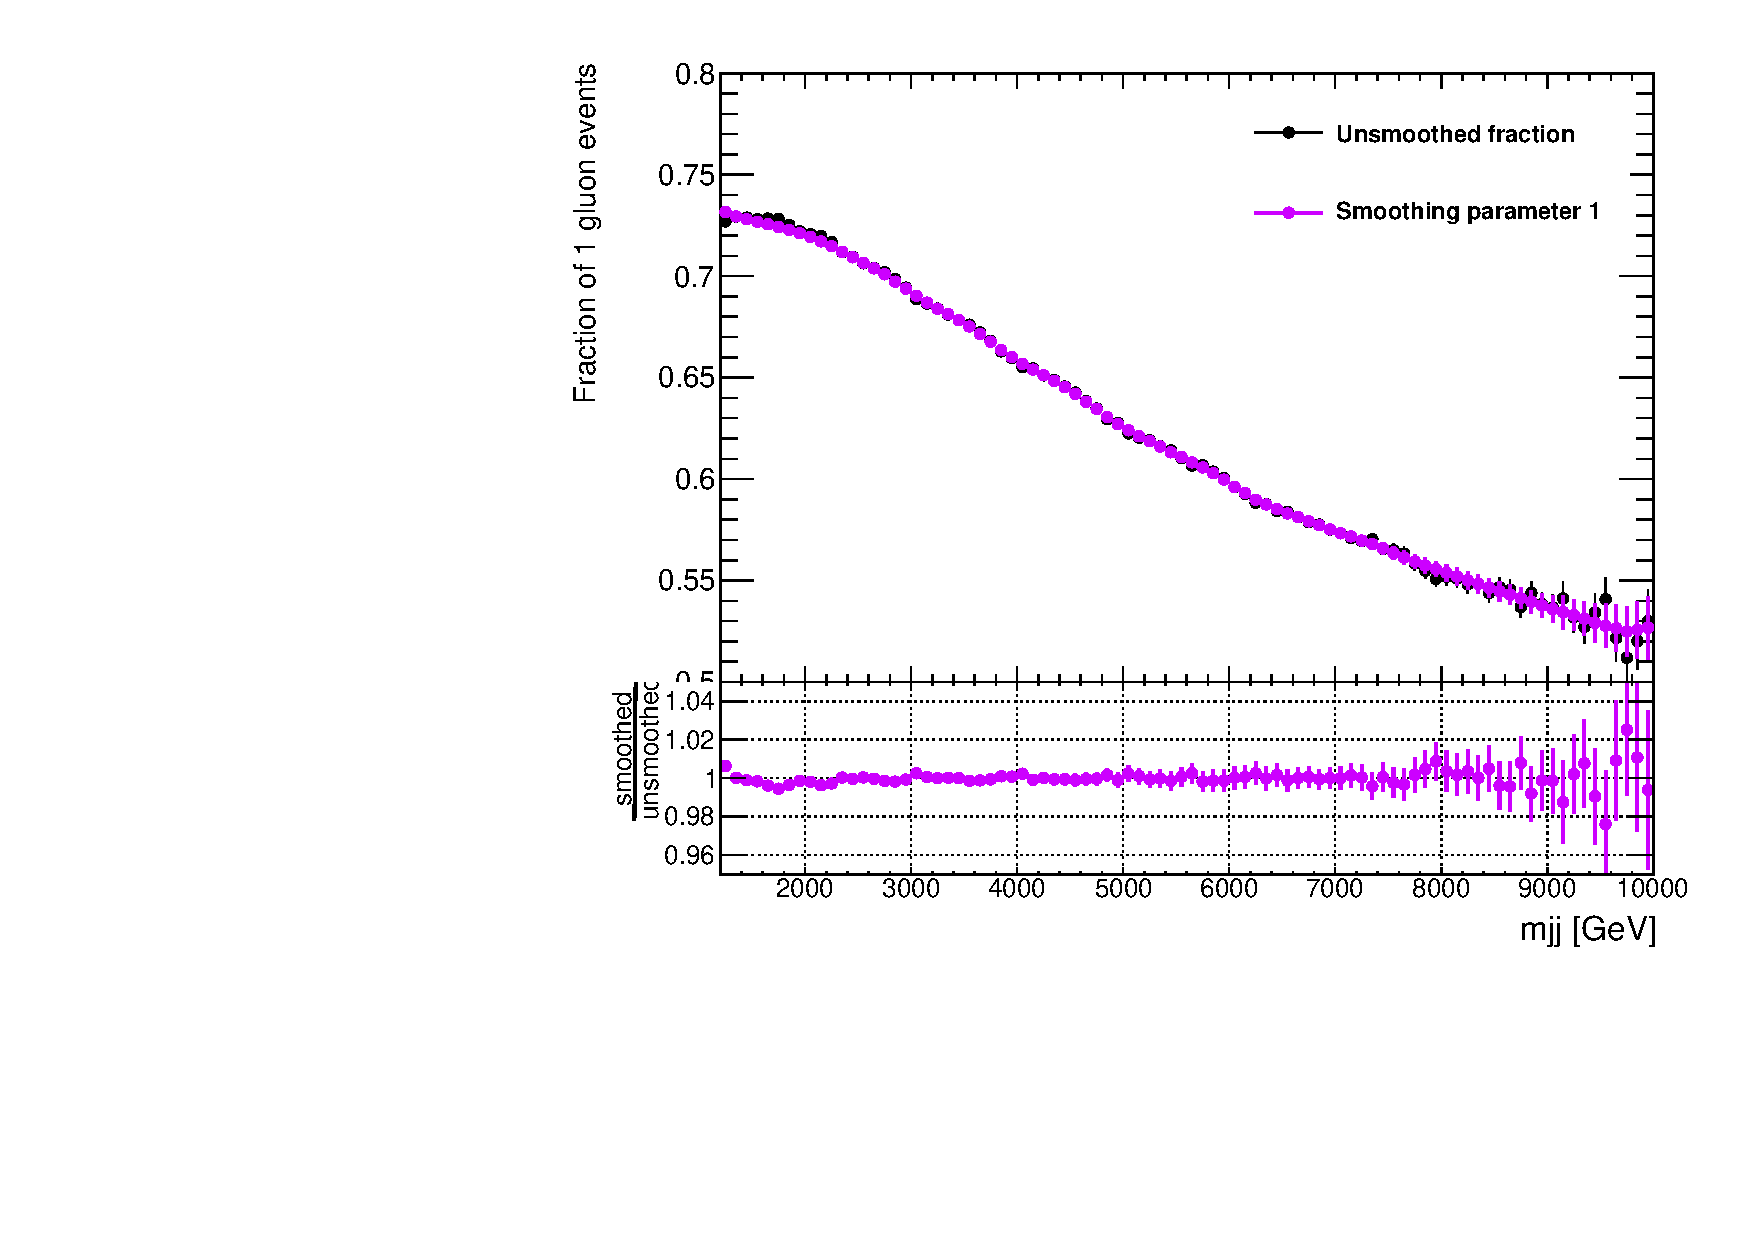
\includegraphics[width=0.48\columnwidth]{figures/pseudodata/Fraction_1gluon_Alpha1to0}}
        \subfigure[Smoothing parameter 7]{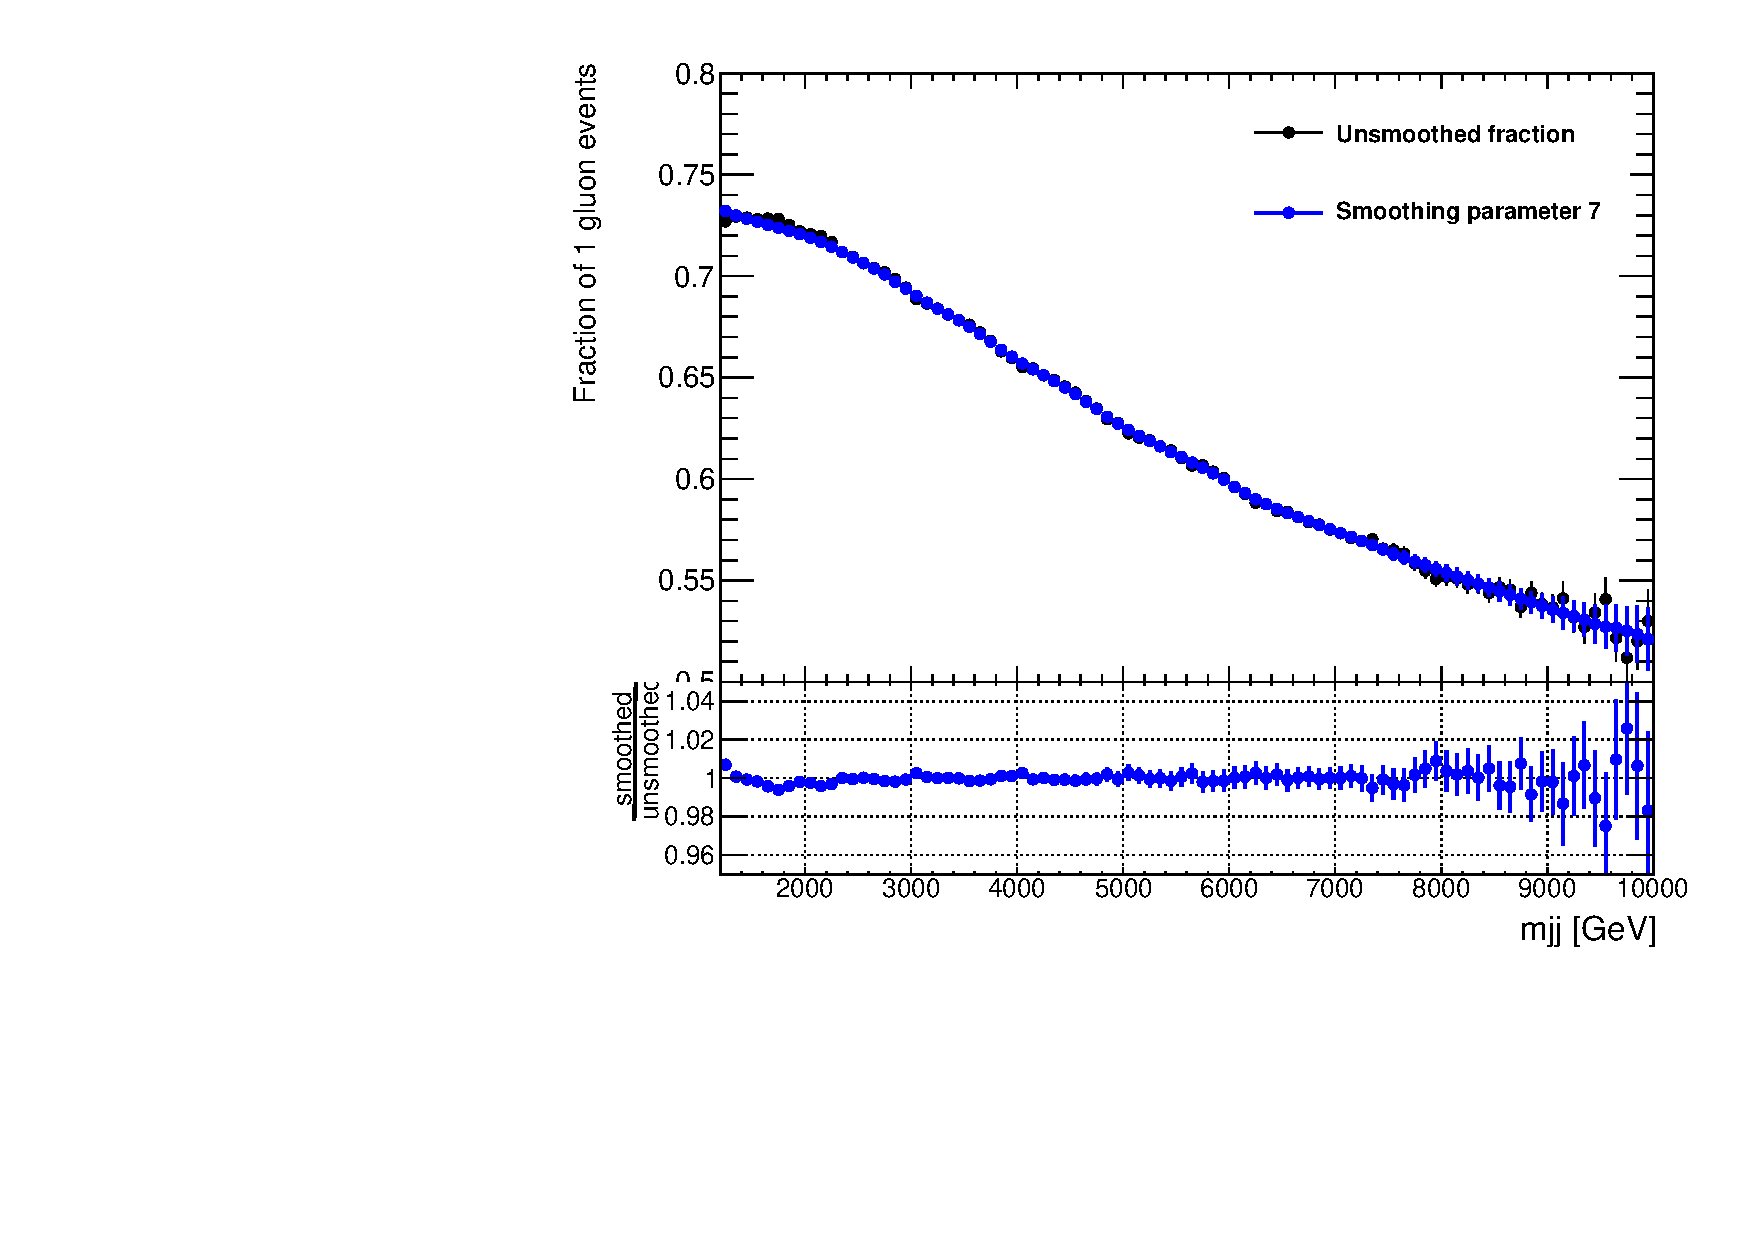
\includegraphics[width=0.48\columnwidth]{figures/pseudodata/Fraction_1gluon_Alpha7to0}}
        \\
        \subfigure[Smoothing parameter 8]{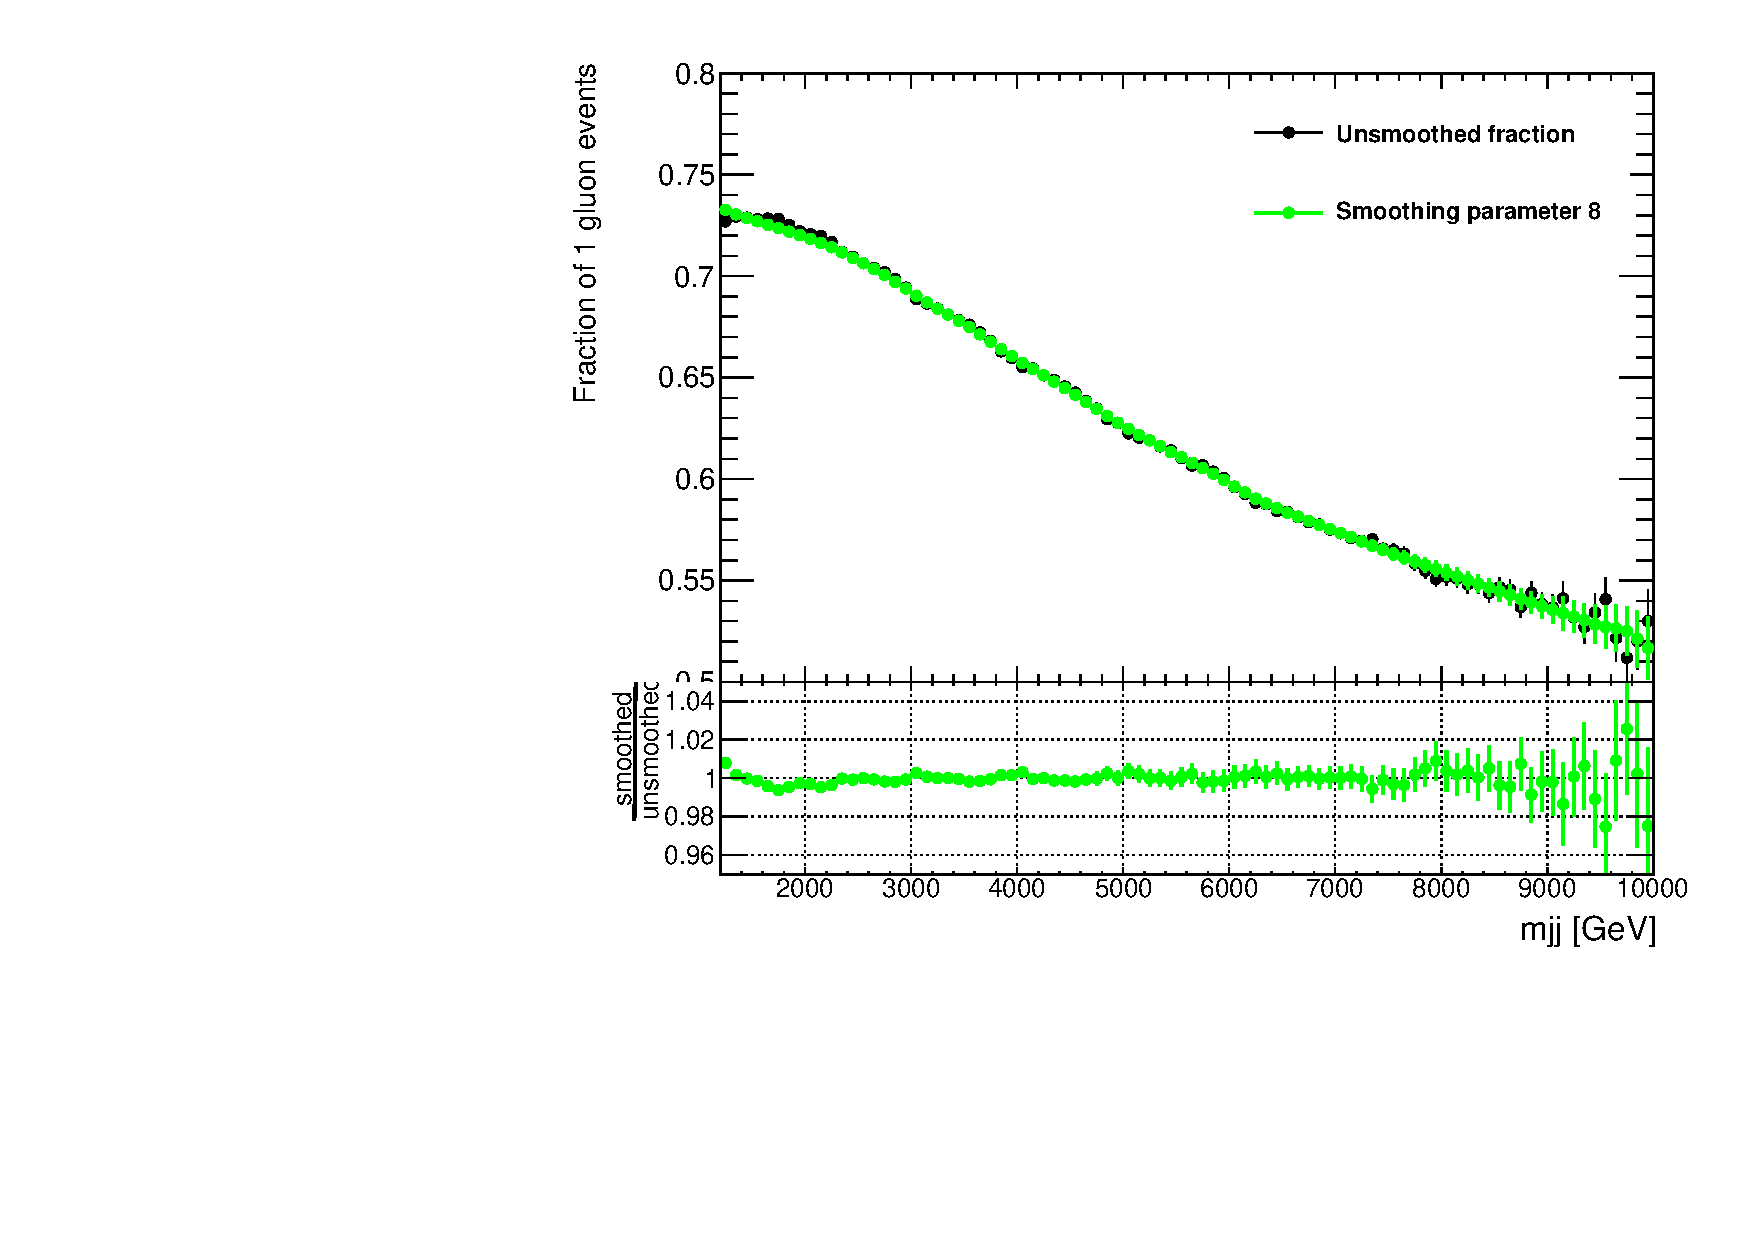
\includegraphics[width=0.48\columnwidth]{figures/pseudodata/Fraction_1gluon_Alpha8to0}}
        \subfigure[Smoothing parameter 10]{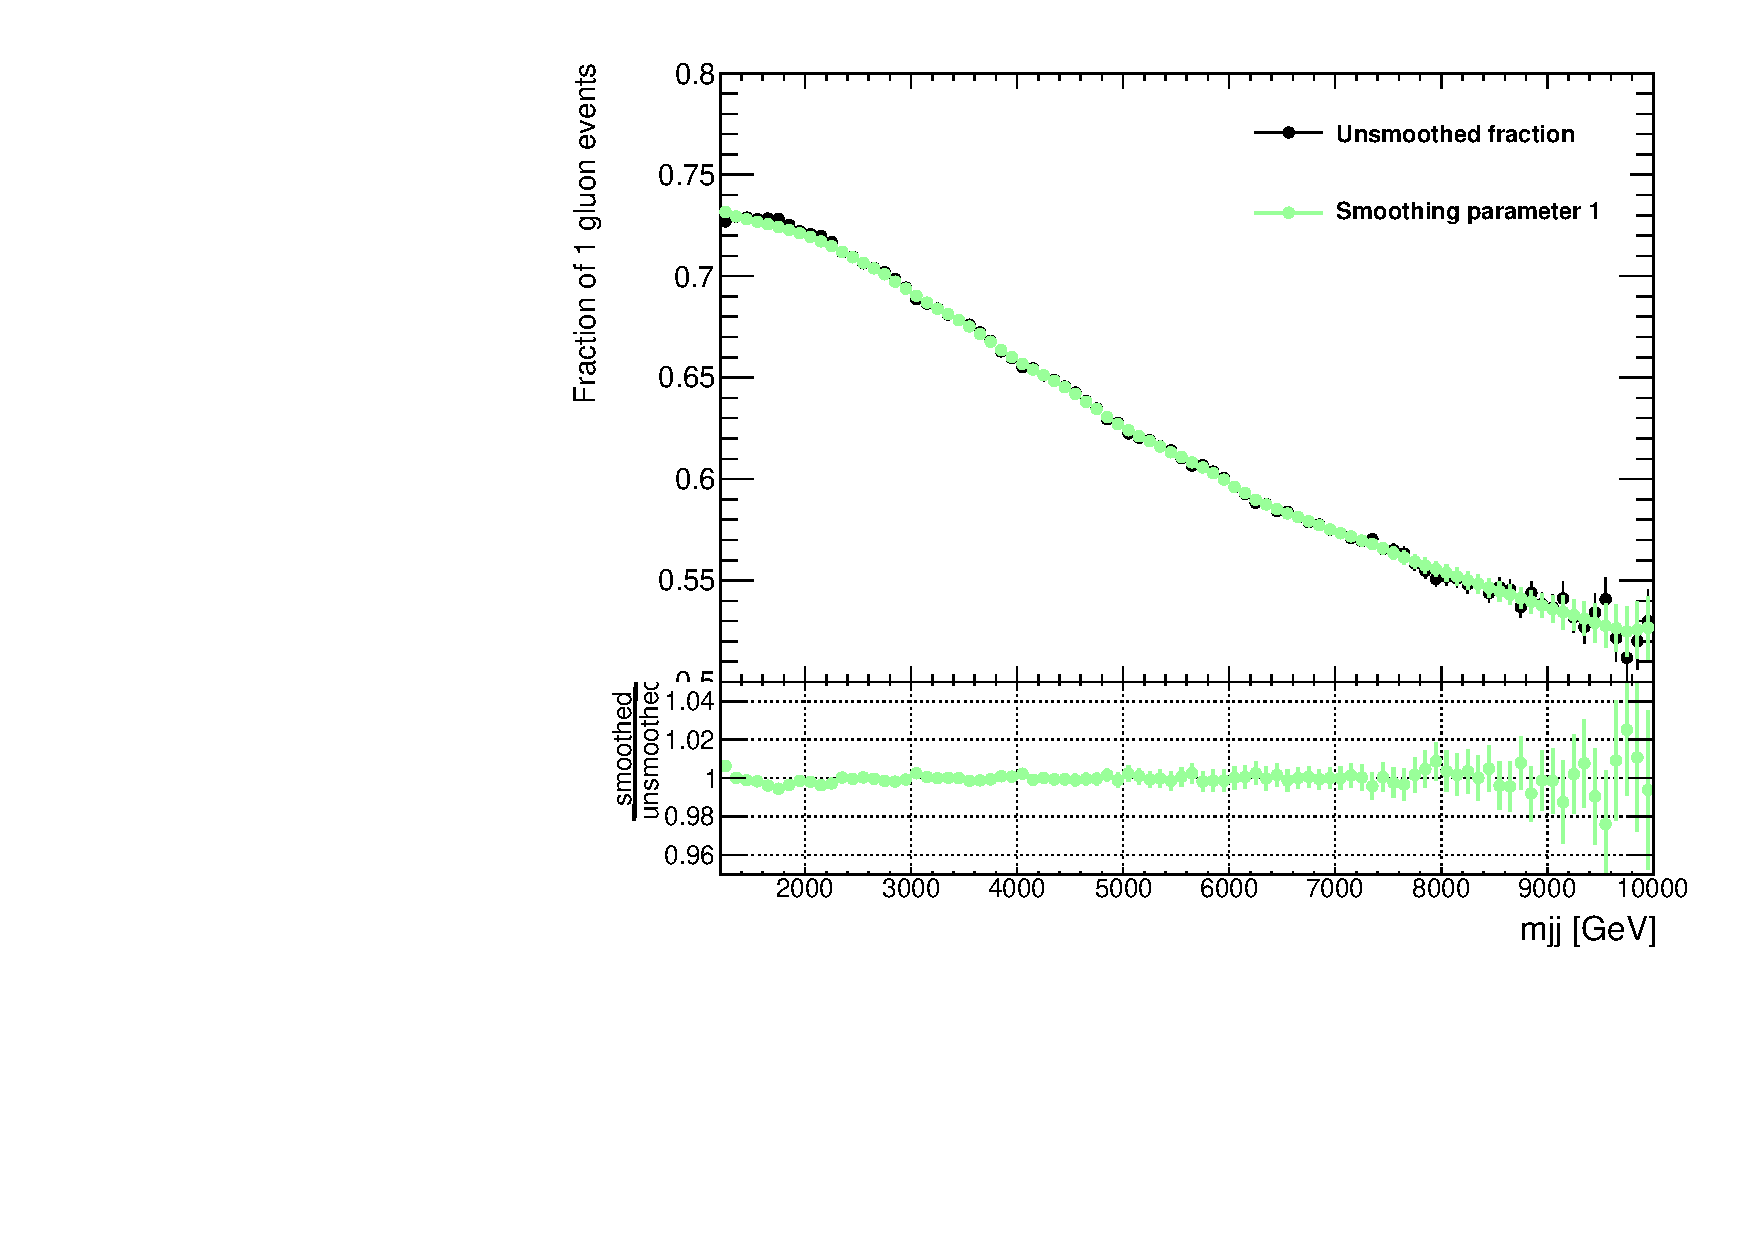
\includegraphics[width=0.48\columnwidth]{figures/pseudodata/Fraction_1gluon_Alpha10to0}}

        \caption{Smoothed fraction of events passing 1 gluon tag selection using smoothing parameter of
        (a) 1 (b) 7 (c) 8 and (d) 10.}
        \label{fig:smoothFractions_1gtag}
\end{figure}

The pseudo-data generated for the 1 gluon tag category can be seen in Figure~\ref{fig:pseudodata_1gtag}.

 \begin{figure}[!htb]
   \centering
   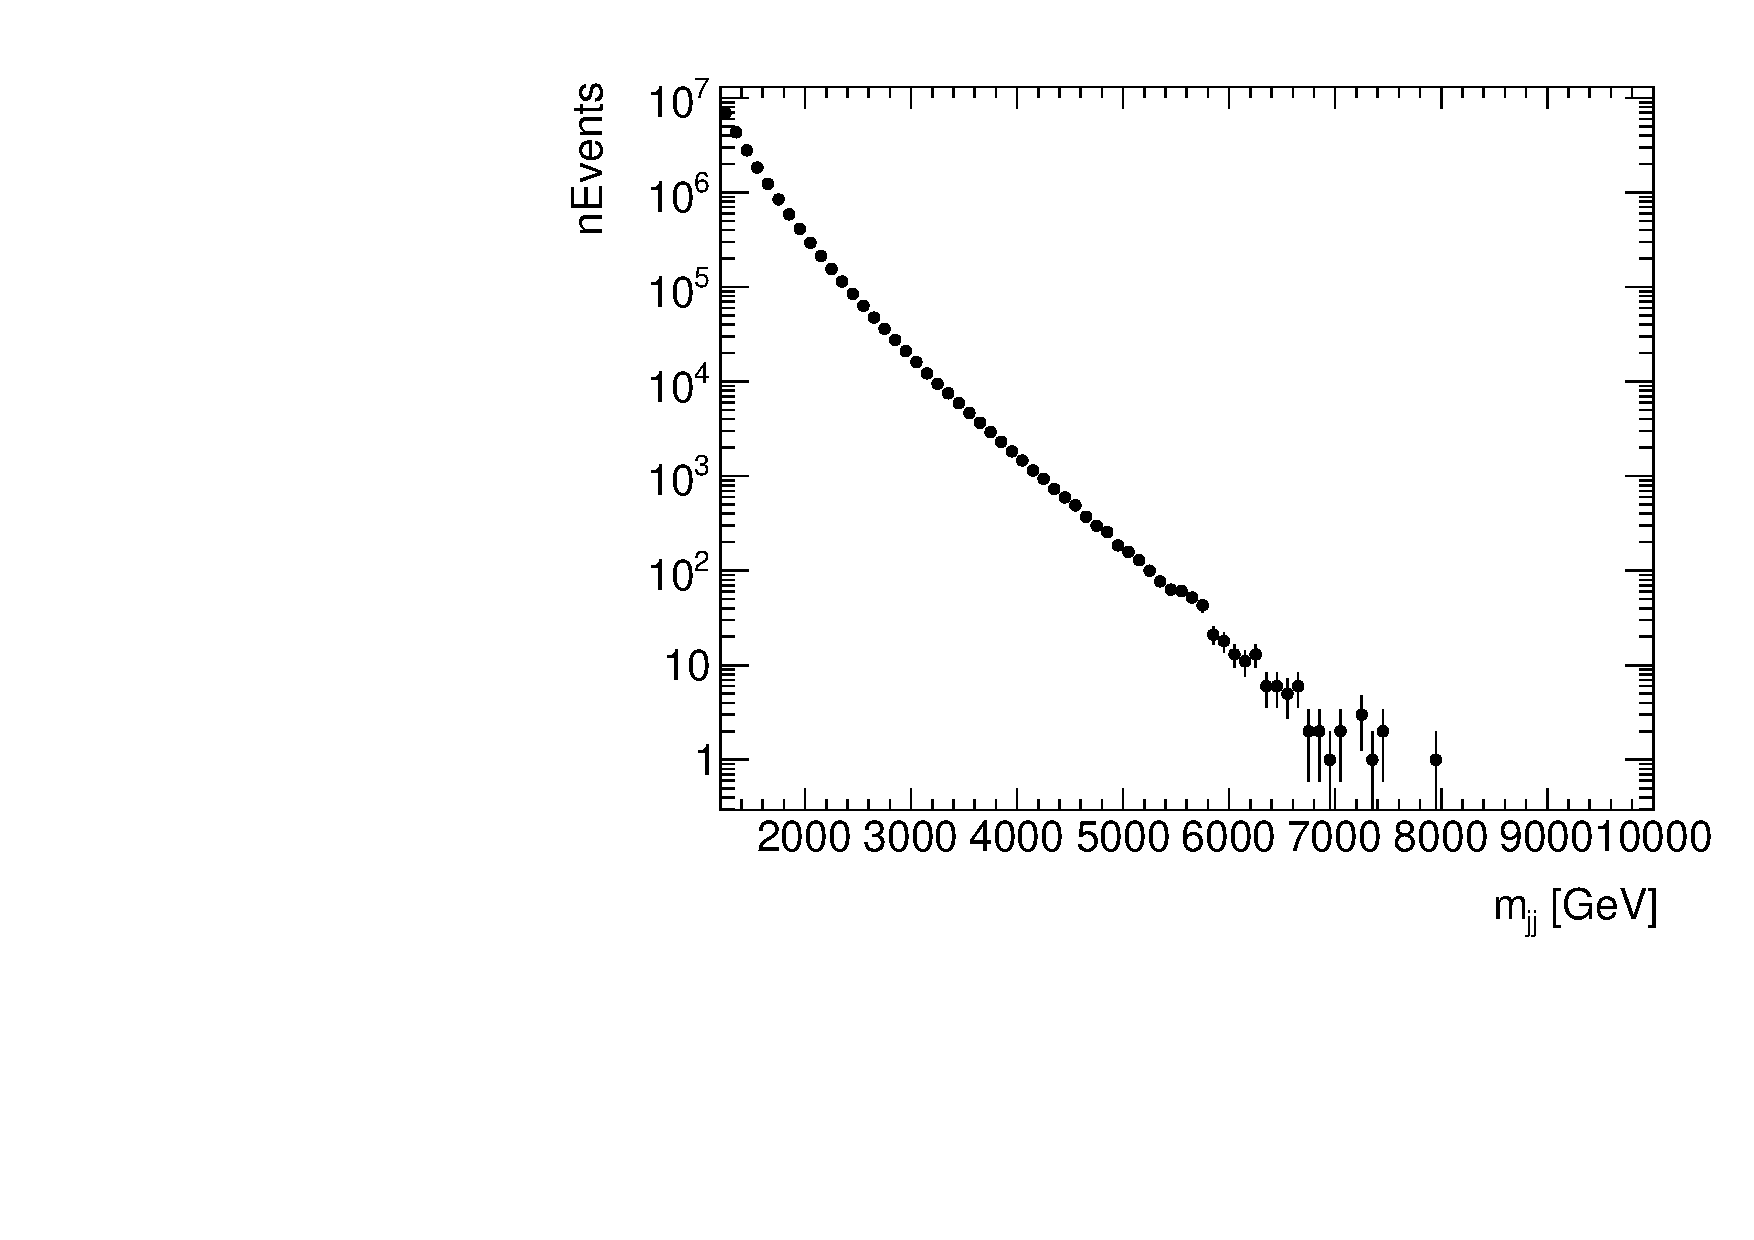
\includegraphics[width=0.45\textwidth]{figures/pseudodata/Pseudodata_1gluonTag.pdf}
   \caption{Pseudodata for 1 gluon tag category.
   \label{fig:pseudodata_1gtag}}
 \end{figure}

Same procedure was followed to obtain the pseudo-data for the 2 gluon tag category using $|\ystar|<0.6$ and \mjj\ > 1100\,\GeV. 
Figure~\ref{fig:mjjFit_ystar0p6} shows the fitted untagged spectrum with 5 parameter global fit using Minuit2 and figure~\ref{fig:fraction_2gtag_unsmooth} shows the fraction of events passing 2 gluon tag selection.
Figure~\ref{fig:smoothFractions_2gtag} shows the smoothed fraction of events passing two gluon tag selection along with the ratios to the unsmoothed fractions. The pseudo-data 
generated for the 2 gluon tag category can be seen in Figure~\ref{fig:pseudodata_2gtag}.

 \begin{figure}[!htb]
   \centering
   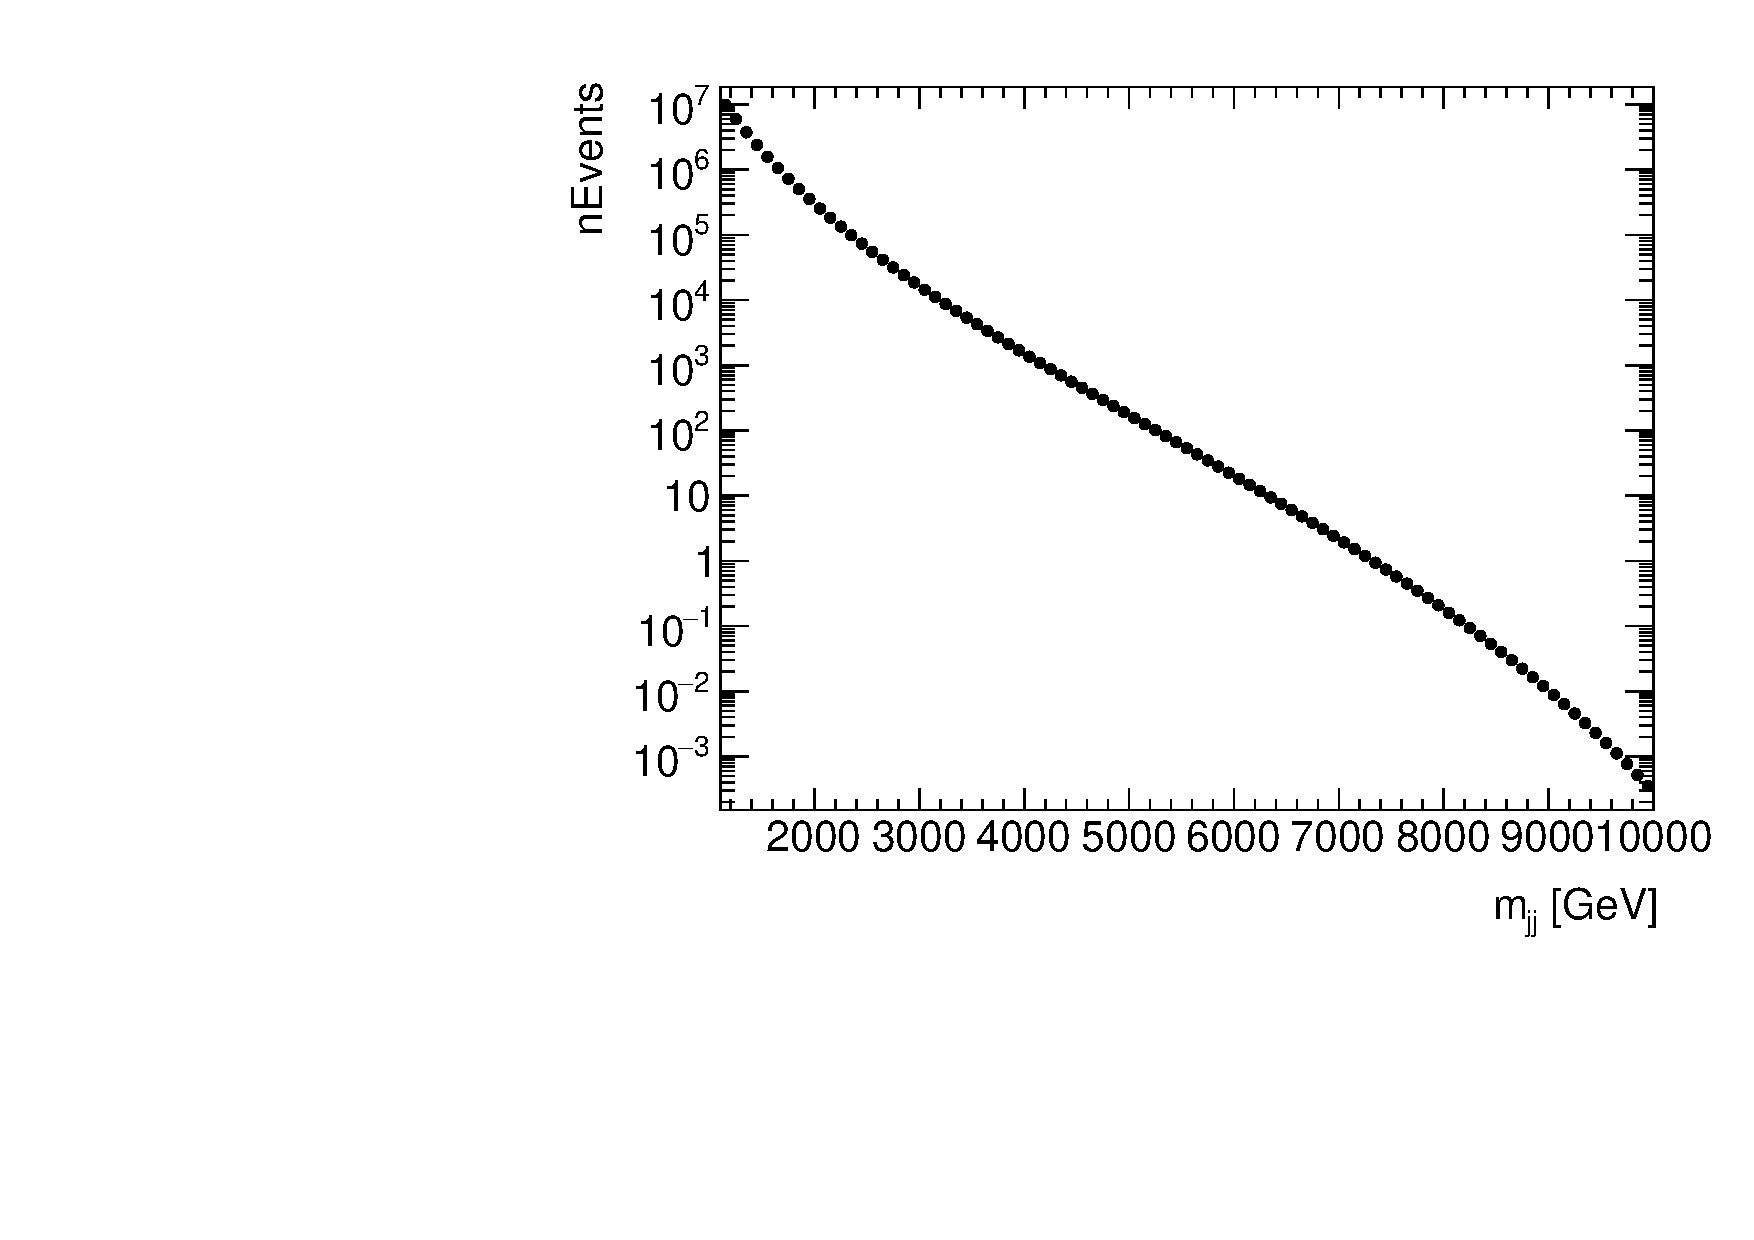
\includegraphics[width=0.45\textwidth]{figures/pseudodata/FittedMjj_UntaggedData_yStar0p6}
   \caption{Untagged dijet spectrum with $|\ystar|<0.6$ using Full Run-2 data fitted with 5 parameter global fit.
   \label{fig:mjjFit_ystar0p6}}
 \end{figure}

 \begin{figure}[!htb]
   \centering
   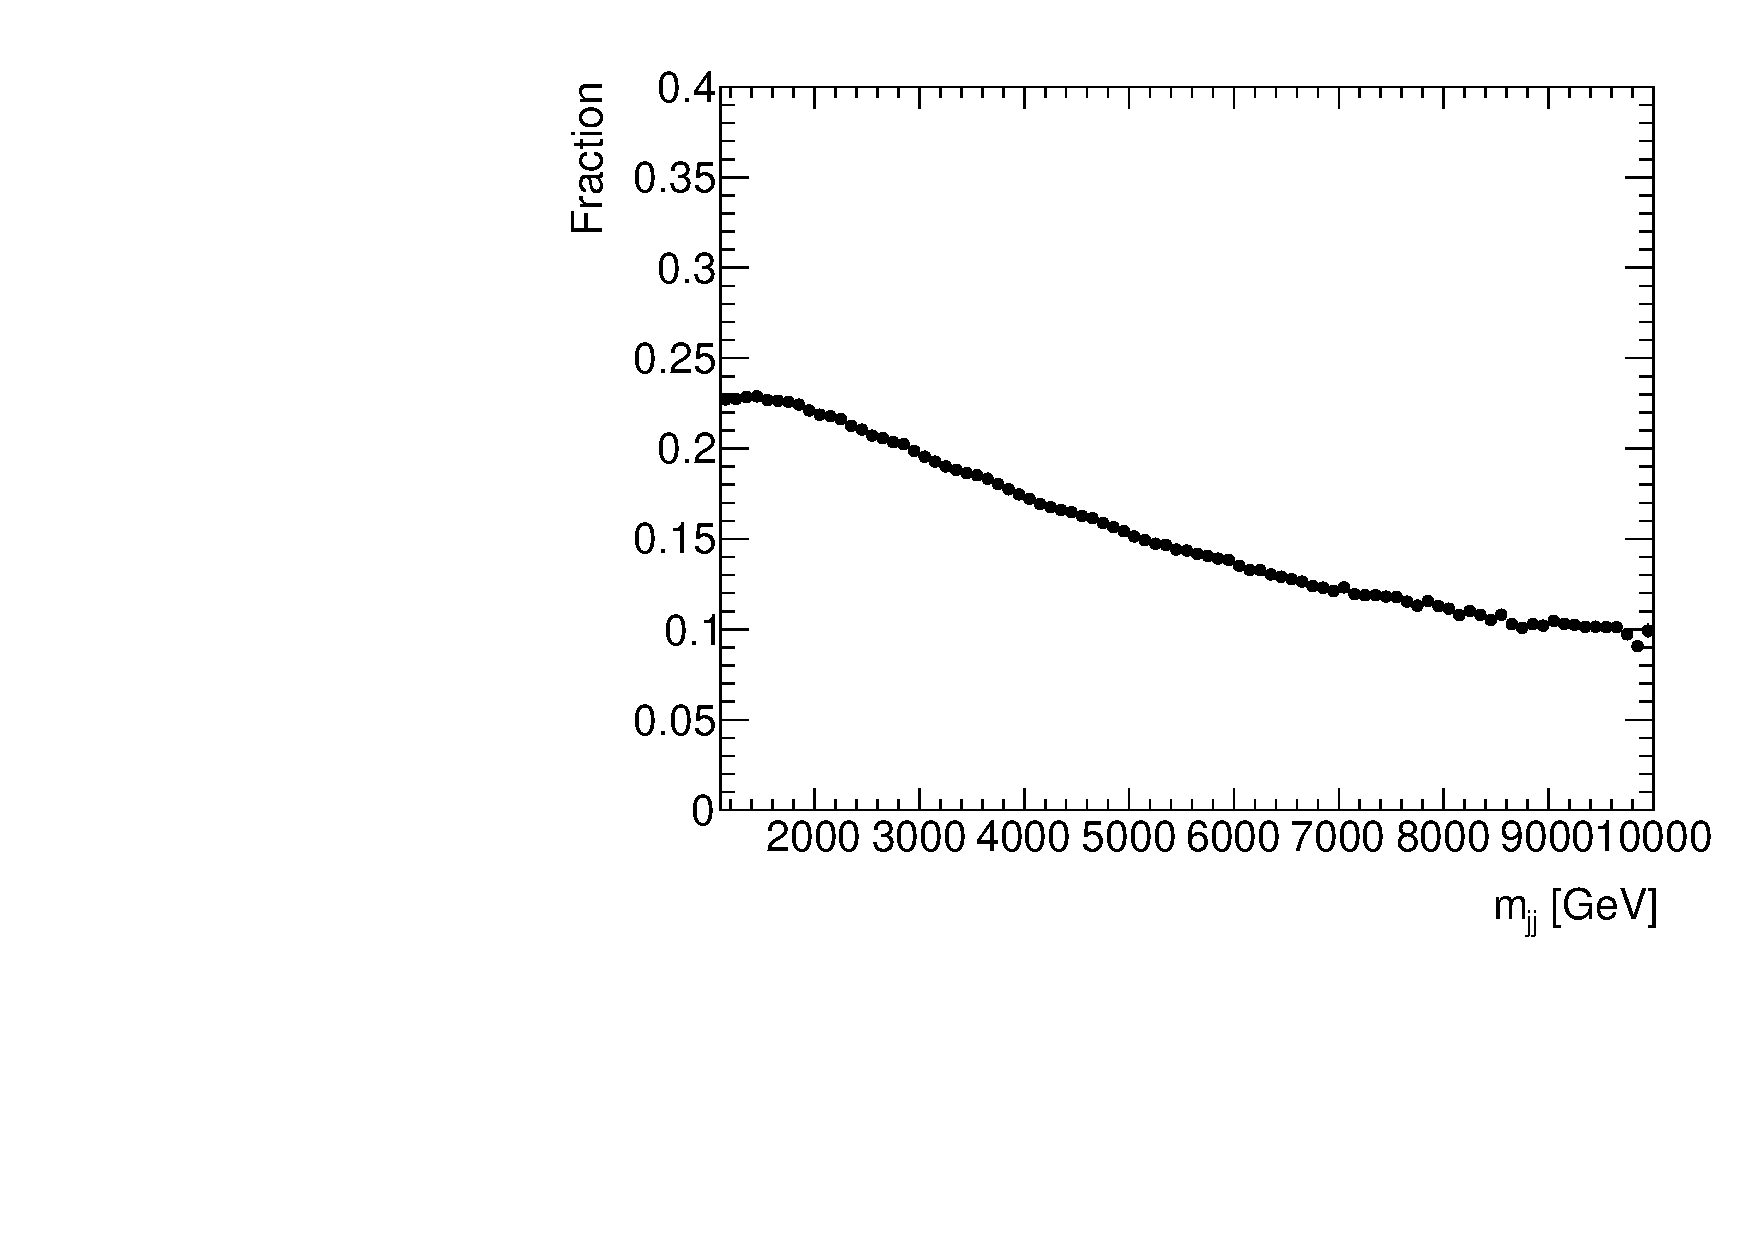
\includegraphics[width=0.45\textwidth]{figures/pseudodata/FractionUnsmooth_2gtag_yStar0p6}
   \caption{Fraction of events passing 2 gluon tag selection.
   \label{fig:fraction_2gtag_unsmooth}}
 \end{figure}


\begin{figure}[htbp]
        \centering
        \subfigure[Smoothing parameter 4]{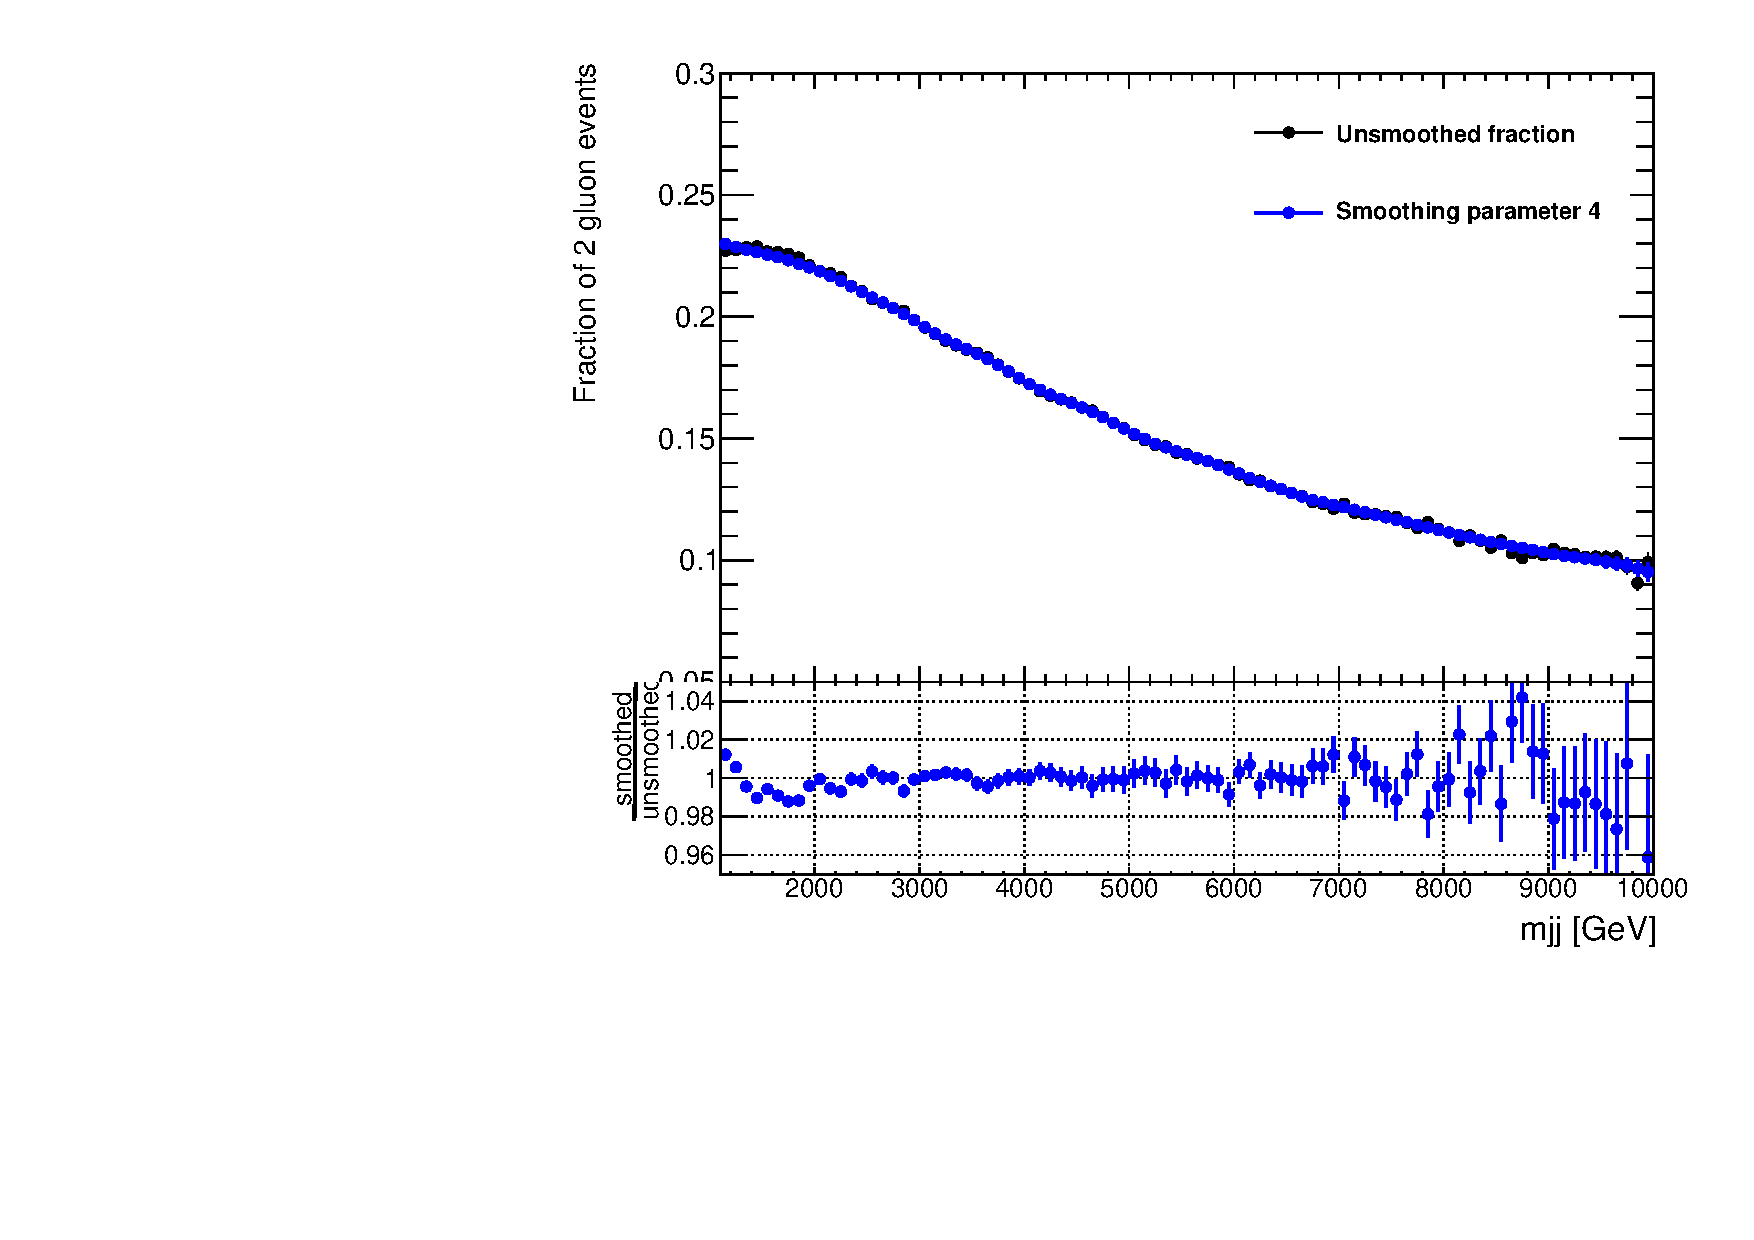
\includegraphics[width=0.48\columnwidth]{figures/pseudodata/Fraction_2gluon_Alpha4to0}}
        \subfigure[Smoothing parameter 6]{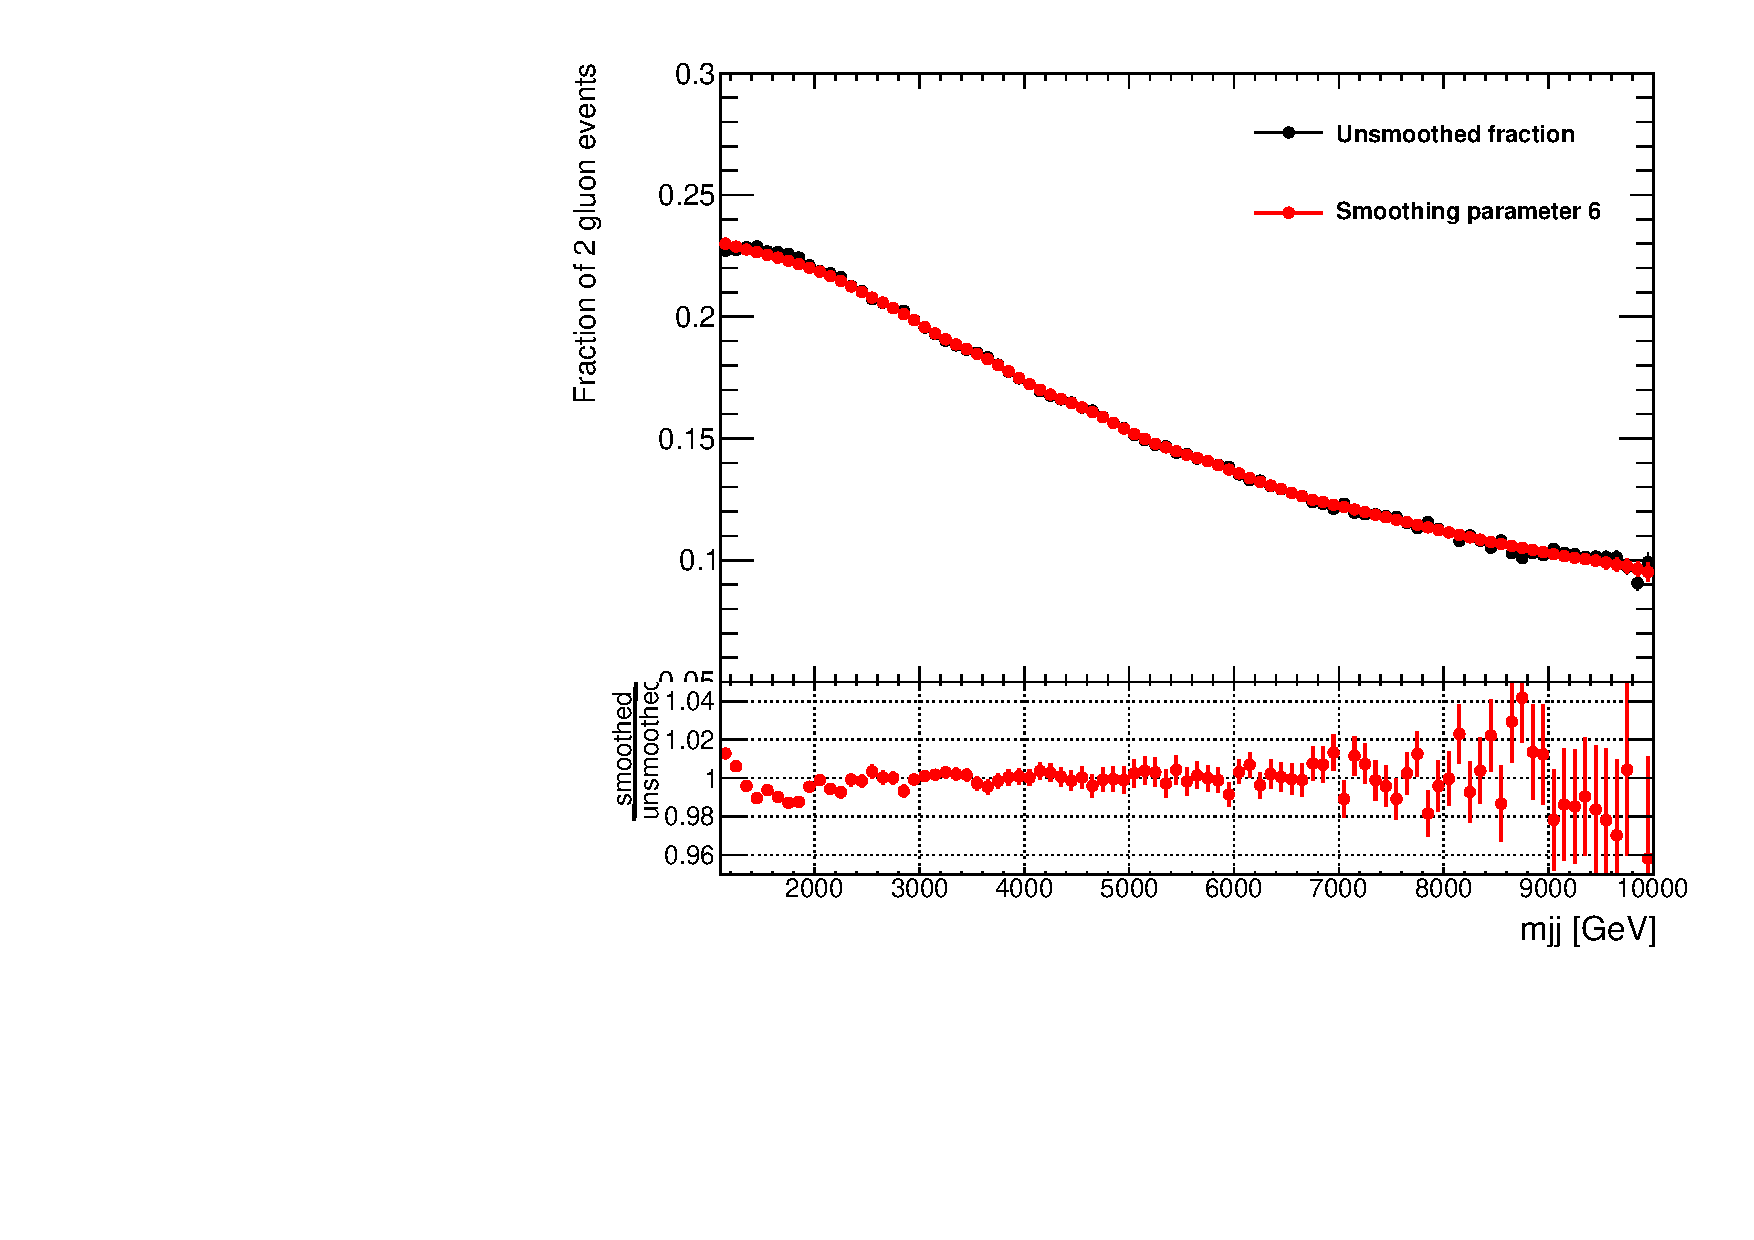
\includegraphics[width=0.48\columnwidth]{figures/pseudodata/Fraction_2gluon_Alpha6to0}}
        \\
        \subfigure[Smoothing parameter 8]{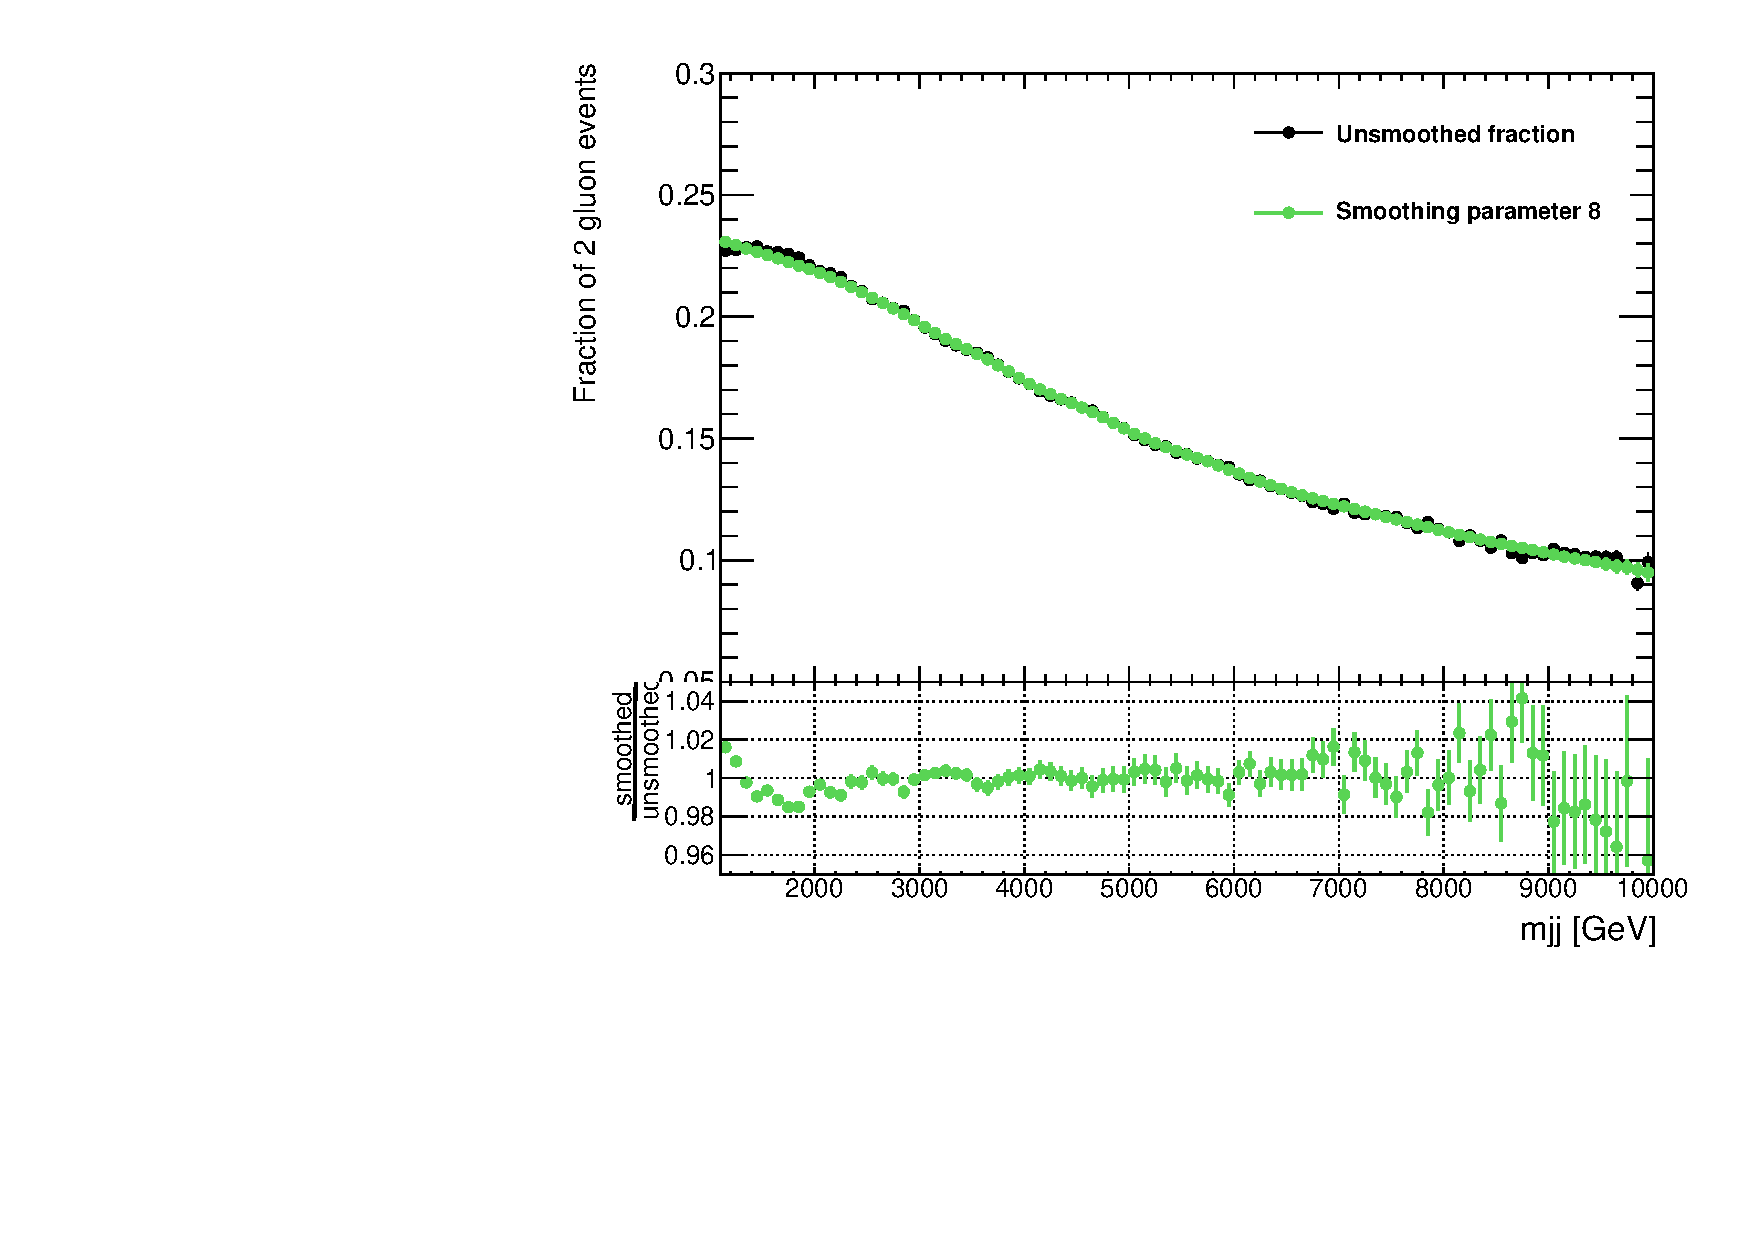
\includegraphics[width=0.48\columnwidth]{figures/pseudodata/Fraction_2gluon_Alpha8to0}}
        \subfigure[Smoothing parameter 10]{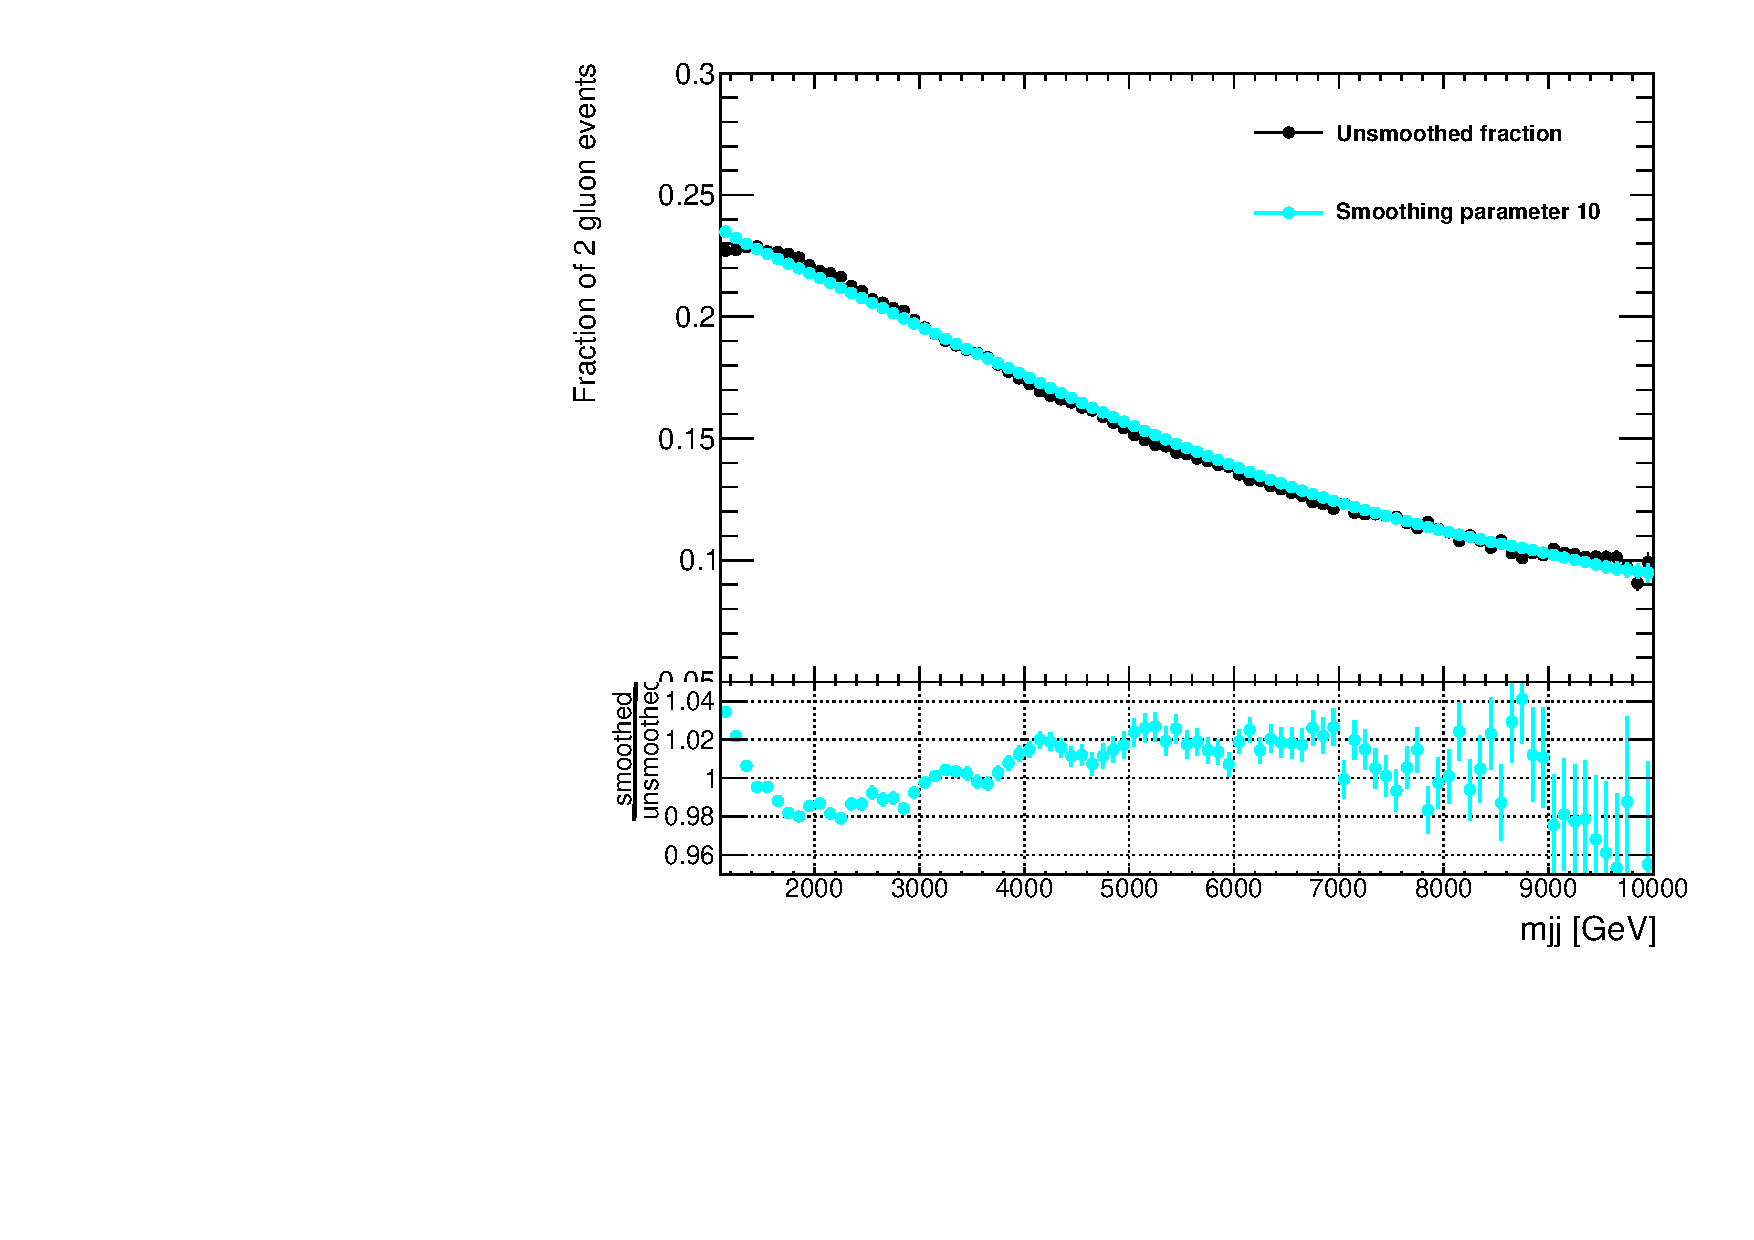
\includegraphics[width=0.48\columnwidth]{figures/pseudodata/Fraction_2gluon_Alpha10to0}}
        \caption{Smoothed fraction of events passing 2 gluon tag selection using smoothing parameter of
        (a) 4 (b) 6 (c) 8 and (d) 10.}
        \label{fig:smoothFractions_2gtag}
\end{figure}

 \begin{figure}[!htb]
   \centering
   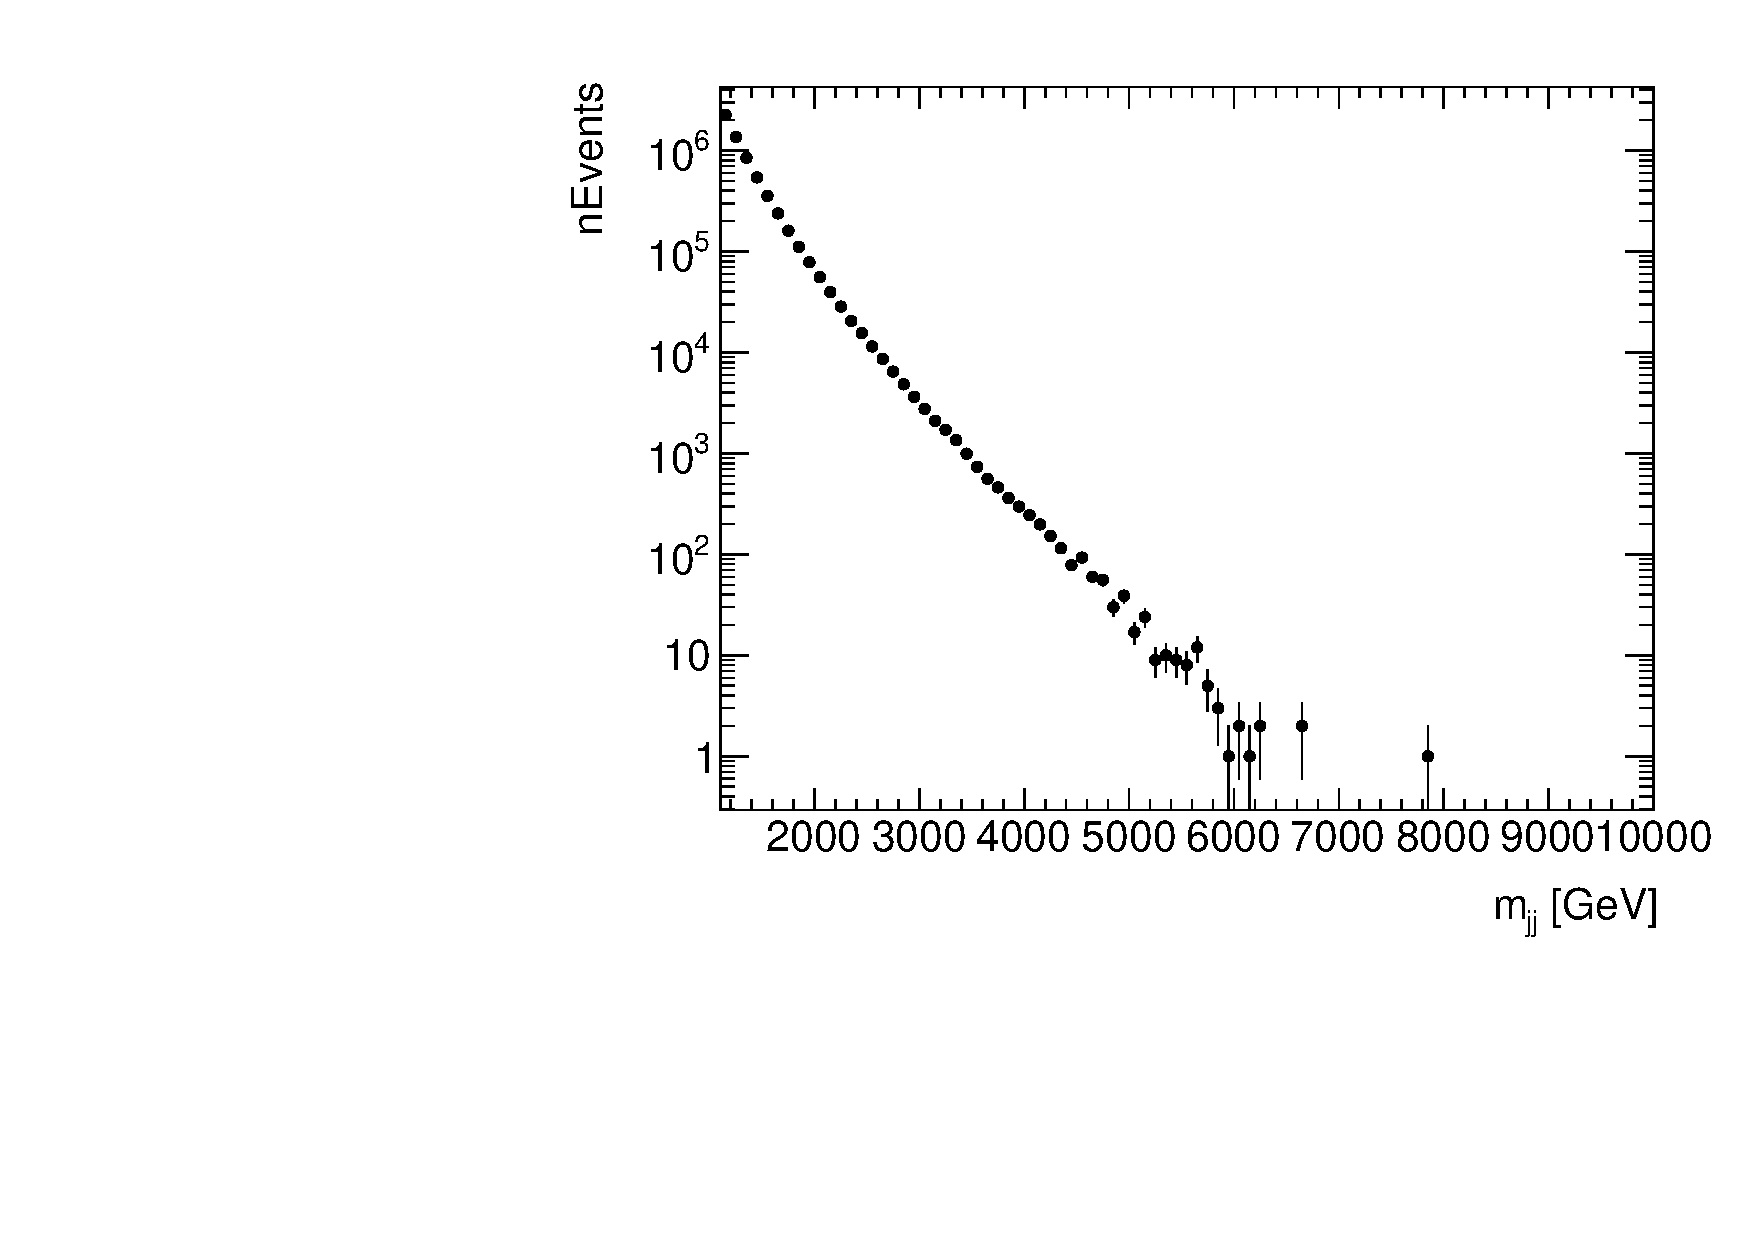
\includegraphics[width=0.45\textwidth]{figures/pseudodata/Pseudodata_2gluonTag.pdf}
   \caption{Pseudodata for 2 gluon tag category.
   \label{fig:pseudodata_2gtag}}
 \end{figure}




